% 2010 年陕西卷文科第 4 题：样本 A、B 的折线图（纵轴为样本值，横轴为 n）。
% 来源 PDF：普通高考/2010/2010陕西文.pdf，SHA-256 428bcb4aee4c6a7a6a9c9d0dca1377b14112594015d1d50a931e725ae0c5c130。
% 原页：第 1 页（A3 三栏）第 1 栏中部，书页码 625。
% 重绘依据：照原页——左图标题 A、右图标题 B；两图均为方格纸，纵轴标 5、10、15，
%   横轴标 0、2、4、6 并在末端加箭头标 n；方格为正方形，横轴每 1 个单位一格，
%   纵轴每 2.5 个单位一格（故 5、10、15 隔一格标注一次），方格框右、上各多出一格。
%   按原页读点（横轴 n=1,…,6）：图 A 依次为 2.5、10、5、7.5、2.5、10；
%   图 B 依次为 15、10、12.5、10、12.5、10。
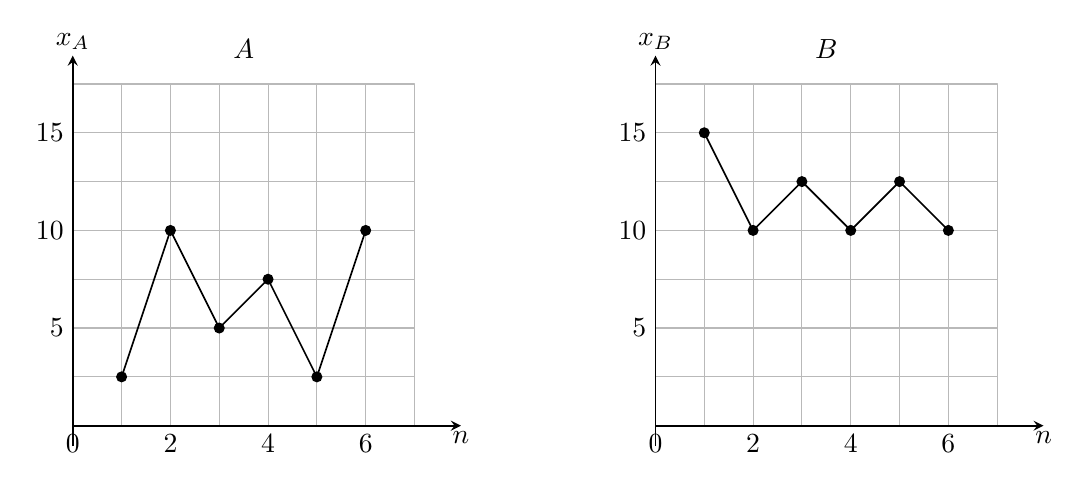
\begin{tikzpicture}[semithick, x=0.62cm, y=0.248cm, line join=round,
  gridl/.style={thin, gray!55}]

  % ================= 图 A =================
  \begin{scope}
    \draw[gridl] (0,0) rectangle (7,17.5);
    \foreach \i in {1,2,3,4,5,6} { \draw[gridl] (\i,0) -- (\i,17.5); }
    \foreach \j in {2.5,5,7.5,10,12.5,15} { \draw[gridl] (0,\j) -- (7,\j); }

    \draw[->, >=stealth] (0,-1.05) -- (0,18.95) node[above, inner sep=2pt] {$x_A$};
    \draw[->, >=stealth] (0,0) -- (7.95,0) node[below, inner sep=2pt] {$n$};

    \foreach \i/\v in {0/0, 2/2, 4/4, 6/6} {
      \node[below, inner sep=3pt] at (\i,0) {$\v$};
    }
    \foreach \j/\v in {5/5, 10/10, 15/15} {
      \node[left, inner sep=3pt] at (0,\j) {$\v$};
    }
    \node at (3.5,19.3) {$A$};

    \draw (1,2.5) -- (2,10) -- (3,5) -- (4,7.5) -- (5,2.5) -- (6,10);
    \foreach \p in {(1,2.5), (2,10), (3,5), (4,7.5), (5,2.5), (6,10)} {
      \fill \p circle (2.0pt);
    }
  \end{scope}

  % ================= 图 B =================
  \begin{scope}[xshift=7.40cm]
    \draw[gridl] (0,0) rectangle (7,17.5);
    \foreach \i in {1,2,3,4,5,6} { \draw[gridl] (\i,0) -- (\i,17.5); }
    \foreach \j in {2.5,5,7.5,10,12.5,15} { \draw[gridl] (0,\j) -- (7,\j); }

    \draw[->, >=stealth] (0,-1.05) -- (0,18.95) node[above, inner sep=2pt] {$x_B$};
    \draw[->, >=stealth] (0,0) -- (7.95,0) node[below, inner sep=2pt] {$n$};

    \foreach \i/\v in {0/0, 2/2, 4/4, 6/6} {
      \node[below, inner sep=3pt] at (\i,0) {$\v$};
    }
    \foreach \j/\v in {5/5, 10/10, 15/15} {
      \node[left, inner sep=3pt] at (0,\j) {$\v$};
    }
    \node at (3.5,19.3) {$B$};

    \draw (1,15) -- (2,10) -- (3,12.5) -- (4,10) -- (5,12.5) -- (6,10);
    \foreach \p in {(1,15), (2,10), (3,12.5), (4,10), (5,12.5), (6,10)} {
      \fill \p circle (2.0pt);
    }
  \end{scope}
\end{tikzpicture}
